Initially, we designed HTBAC to implement a single binding affinity protocol,
using the EnTK programming model to express the application logic. Here, we
exclusively focus on ESMACS to capture the workflow logic and isolate the
performance of a single protocol instance. HTBAC has been extended as a
Python library that enables the selection of multiple protocol instances of
ESMACS and TIES~\cite{dakka}.

A simulation pipeline is a defined sequence of simulation stages for a given
physical system. In the ESMACS protocol, these simulation pipelines are
replicated, where replicas differ only by their parameter configurations,
namely initial velocities, which are randomly generated and assigned by NAMD
at the start of execution. A simulation pipeline in the ESMACS protocol has 7
stages: the first, second and last stages perform staging of the input/output
data, the middle stages indicate simulation tasks. A task is appended to a
stage and stages are appended to a pipeline to maintain temporal order during
execution.

% The ESMACS protocol performs a sequence of simulation stages for a given
% physical system. ESMACS replicates this sequence of simulation stages.
% Replicas differ only by their parameter configurations, namely initial
% velocities, which are randomnly generated and assigned by NAMD at the start
% of execution.

% \begin{figure}[h!]
% \caption{\csentence{ESMACS Implementation using EnTK.}
%   ESMACS protocol implemented as an ensemble application, encoded
%   using the EnTK API\@. A protocol represents a physical system and is
%   encoded as a set of independent pipelines. Each pipeline maps to a single
%   replica. ESMACS consists of 25 replicas. Stages within a pipeline are
%   executed sequentially. Each stage contain a single task performing unique
%   functions, as required by the protocol. Stages S3--S6 contain molecular
%   dynamics simulation tasks executed with NAMD\@.}
%   %\jhanote{Can we chat about this schematic? fixed}}
%   \label{figure:HTBAC}
%   \end{figure}

\begin{figure}
\centering
  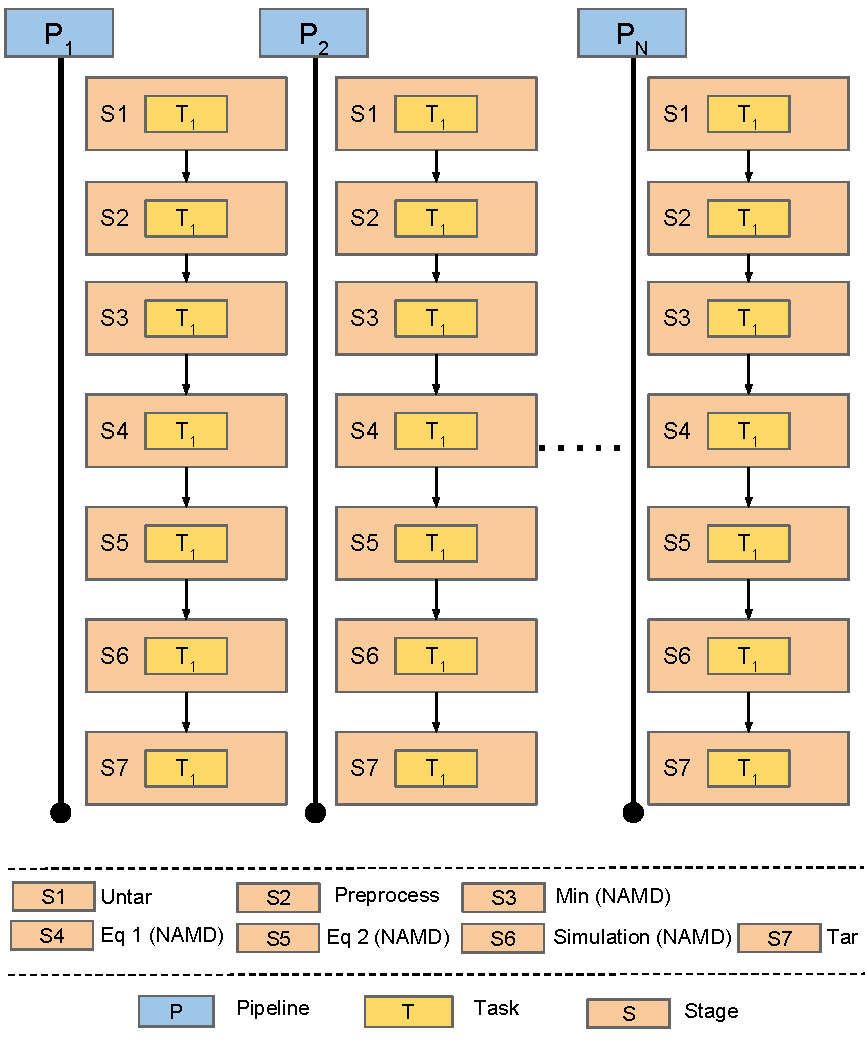
\includegraphics[width=0.4\textwidth]{HTBAC_Workflow_ESMACS.pdf}
  \caption{ESMACS protocol implemented as an ensemble application, encoded
  using the EnTK API\@. A protocol represents a physical system and is
  encoded as a set of independent pipelines. Each pipeline maps to a single
  replica. ESMACS consists of 25 replicas. Stages within a pipeline are
  executed sequentially. Each stage contain a single task performing unique
  functions, as required by the protocol. Stages S3--S6 contain molecular
  dynamics simulation tasks executed with NAMD}
  \label{figure:HTBAC}
\end{figure}


Each simulation pipeline replica maps to an independent EnTK pipeline. Each
pipeline consists of a sequence of stages, and each stage consists of a single
task that performs unique functions, including pre-processing and molecular
dynamics simulations. Fig~\ref{figure:HTBAC} shows how pipelines, stages and
tasks are organized for the ESMACS protocol. A task is composed of a set of
attributes that define parameters like the location of input files, the number
of simulations and the MD engine(s) used to launch those simulations.


% \begin{figure}[h!]
% \caption{\csentence{ESMACS-EnTK-RP Integration.}
%   Integration between ESMACS and EnTK\@. Numbers indicate
%   the temporal sequence of execution. The database (DB) of RADICAL-Pilot (RP)
%   can be deployed on any host reachable from the resources. RP pushes compute
%   units (CU) to DB and pulls them for execution.}
%   \label{figure:ht-bac_rp}
%   \end{figure}


\begin{figure}
\centering
  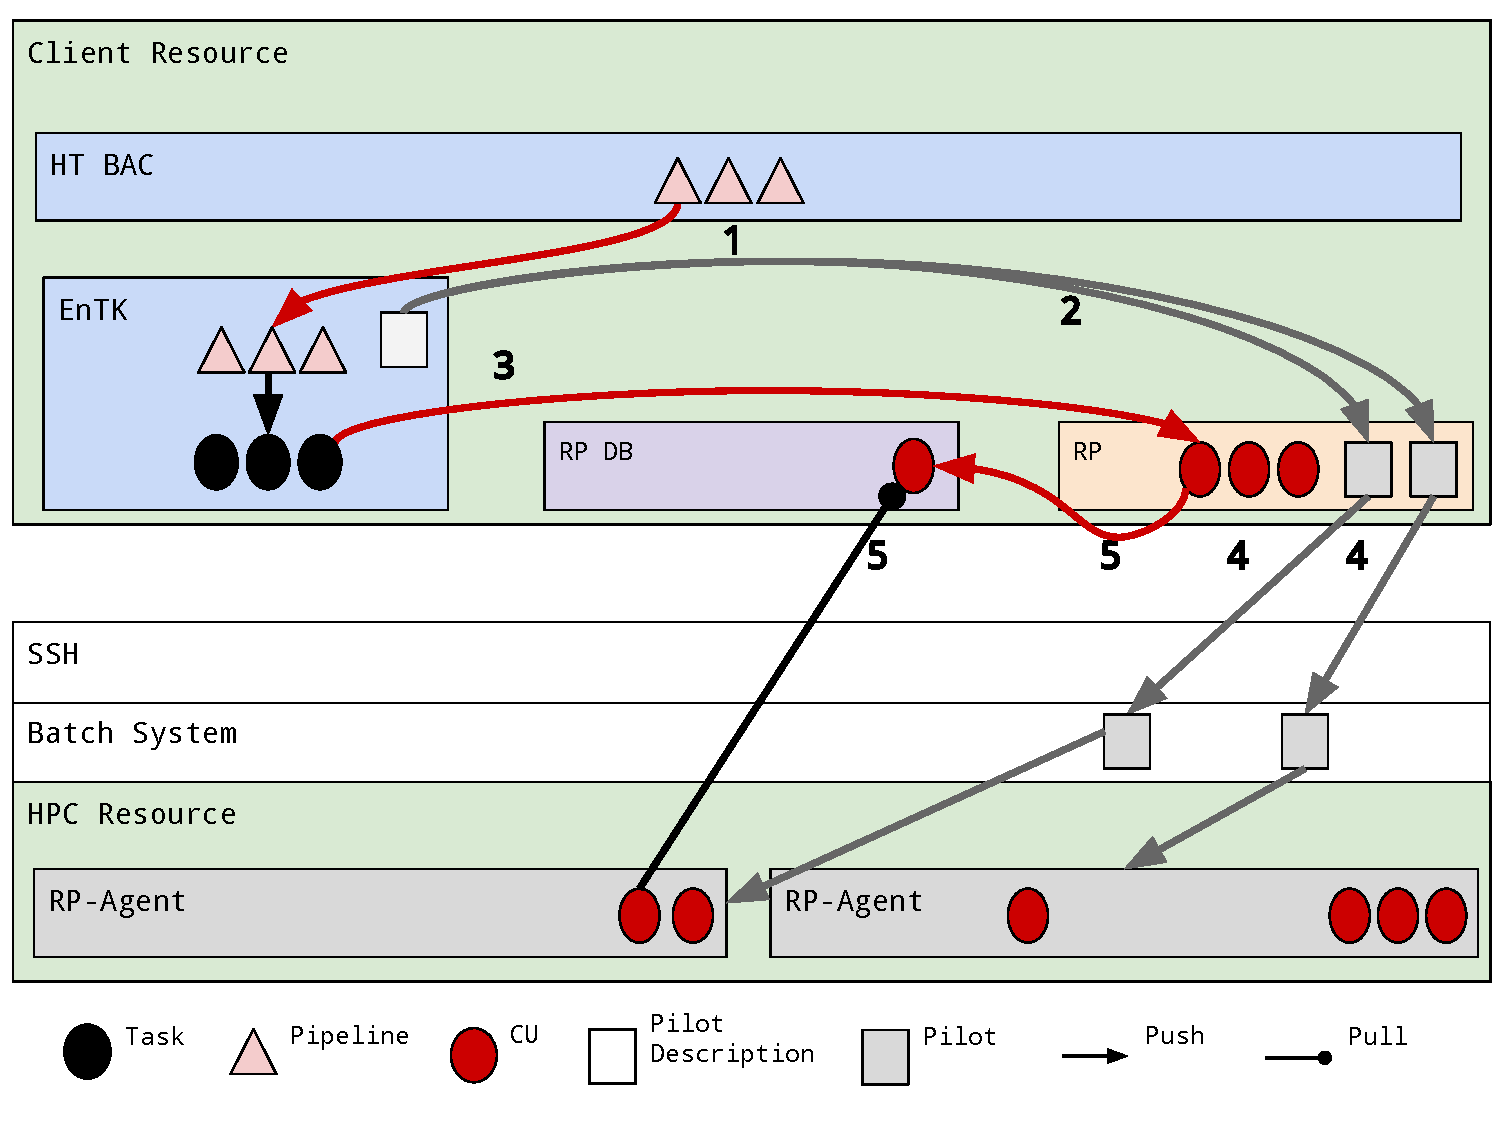
\includegraphics[width=0.5\textwidth]{ht-bac-rp_integration.pdf}
  \caption{ESMACS-EnTK-RP Integration.
  Integration between ESMACS and EnTK\@. Numbers indicate
  the temporal sequence of execution. The database (DB) of RADICAL-Pilot (RP)
  can be deployed on any host reachable from the resources. RP pushes compute
  units (CU) to DB and pulls them for execution.}
  \label{figure:ht-bac_rp}
\end{figure}


Fig.~\ref{figure:ht-bac_rp} shows how the ESMACS protocol integrates with
EnTK\@. EnTK converts the set of pipelines into a set of tasks called compute
unit descriptions and submits them to RP\@. In addition, EnTK provides
methods for the user to specify a resource request including walltime, cores,
queue, and user credentials. EnTK converts this resource request into a pilot
that RP submits to a HPC machine. Once the pilot becomes active, it pulls
compute unit descriptions in bulk from a database, executing them on the
pilot resources.